\subsection{UCW5 - Proposta profilo Instagram}
\begin{figure}[!h]
\centering
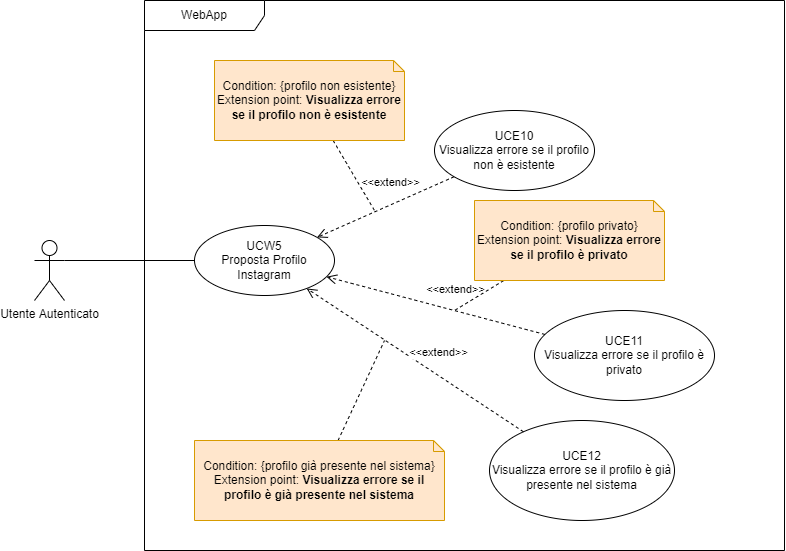
\includegraphics[scale=0.5]{UC_images/UCW5.png}
\caption{UCW5 - Proposta profilo Instagram}
\end{figure}
\begin{itemize}
	\item \textbf{Descrizione}: L'utente autenticato propone uno specifico profilo Instagram da cui effettuare il crawling dei dati.
    \item \textbf{Attore primario}: Utente autenticato.
    \item \textbf{Precondizione}: Il sistema possiede una lista di profili instagram da cui effettuare il crawling dei dati.
    \item \textbf{Postcondizione}: Alla lista di profili da cui effettuare il crawling viene aggiunto il profilo indicato dall’utente e tutti i profili pubblici seguiti dal profilo suggerito.
    \item \textbf{Scenario principale}: 
    \begin{enumerate}
        \item L'utente autenticato accede al sistema;
        \item L’utente seleziona la funzionalità suggerisci un profilo instagram;
        \item L’utente inserisce uno username valido di un profilo instagram pubblico.
    \end{enumerate}
    \item \textbf{Estensioni}:
    \begin{itemize}
        \item Nel caso in cui l’utente inserisca uno username non esistente:
        \begin{enumerate}
            \item Lo username non viene inserito nella lista;
            \item Viene visualizzato un messaggio di errore nella proposta di profilo (UCE10 §3.24);
            \item Viene fornita all’utente la possibilità di modificare lo username inserito.
        \end{enumerate}
        \item Nel caso in cui l’utente inserisca lo username di un profilo privato:
        \begin{enumerate}
            \item Lo username non viene inserito nella lista;
            \item Viene visualizzato un messaggio di errore nella proposta di profilo (UCE11 §3.25).
        \end{enumerate}
        \item Nel caso in cui venga inserito lo username di un profilo pubblico già presente nel sistema:
        \begin{enumerate}
            \item Lo username non viene inserito nella lista.
            \item Viene visualizzato un messaggio di errore nella proposta di profilo (UCE12 §3.26).
        \end{enumerate} 
    \end{itemize}
\end{itemize}

% \subsection{UC3.1 - Verifica privacy profilo}
% \begin{itemize}
%     \item \textbf{Attore primario}: Utente autenticato.
%     \item \textbf{Attore secondario}: Social generico.
%     \item \textbf{Precondizione}: L’utente ha richiesto l’aggiunta di un profilo social fornendone il link.
%     \item \textbf{Postcondizione}: Il sistema sa se il profilo suggerito è pubblico o privato.

%     \item \textbf{Scenario principale}: 
%     \begin{enumerate}
%         \item Il sistema chiede al social in questione se il profilo proposto è pubblico o privato;
%         \item Il social in questione invia una risposta dicendo se il profilo è pubblico o privato.
%     \end{enumerate}

%     \item \textbf{Inclusioni}:
%     \begin{enumerate}
%         \item Verifica validità link (UC3.2 §).
%     \end{enumerate}
% \end{itemize}

% \subsection{UC3.2 - Verifica validità link}
% \begin{itemize}
%     \item \textbf{Attore primario}: Utente autenticato.
%     \item \textbf{Attore secondario}: Social generico.
%     \item \textbf{Precondizione}: L’utente ha richiesto l’aggiunta di un profilo social fornendone il link.
%     \item \textbf{Postcondizione}: Il sistema sa se il link fornito è valido.

%     \item \textbf{Scenario principale}: 
%     \begin{enumerate}
%         \item Il sistema chiede al social in questione se il link è valido;
%         \item Il social in questione invia una risposta dicendo se il link è valido o meno.
%     \end{enumerate}
% \end{itemize}